\subsection{The Selection of Cities}

We survey cohorts of individuals educated in Parma, Padova, and Reggio Emilia. Parma and Padova are similar to Reggio Emilia in terms of geography, population, and socio-economic structure, but they do not have the full Reggio Approach available.\footnote{Other Italian cities were also considered, notably Brescia, Livorno, Modena, Perugia, Piacenza, Prato, and Ravenna. Parma and Padova were the two cities that had social and economic characteristics most similar to Reggio Emilia and were geographically close.}

The cities are in close geographic proximity with Reggio Emilia, which may contribute to the plausibility of spillover effects. Parma is in the same administrative region of Emilia-Romanga. They have similar populations as seen in Figure~\ref{fig:population}. Although the population in Padova is larger than in Parma and Reggio Emilia, the trends are similar across time. The similarity in trends can also be seen in comparing the migration rates among the three cities (Figure~\ref{fig:emigr-immigr}). Although emigration rate is highest in Padova and net migration rate is highest in Reggio Emilia for most of the years, general trends in emigration and immigration are similar in all cities. Levels of foreign immigration are almost identical in the three cities.

The similarities between the cities are also seen in economic terms. Reggio Emilia has an average per-capita income of 25,226 euros, Parma of 28,437, and Padova of 29,915 in 2011 \citep{Comuni-Italiani_2017_Redditi-Ipref-per-Regione-2011}. Other economic information, such as unemployment, is similar across the cities as well. We present additional information on the three cities in Appendix~\ref{sec:data-app}.

\begin{figure}[H]
      \begin{center}
        \begin{subfigure}[t]{0.49\textwidth}
          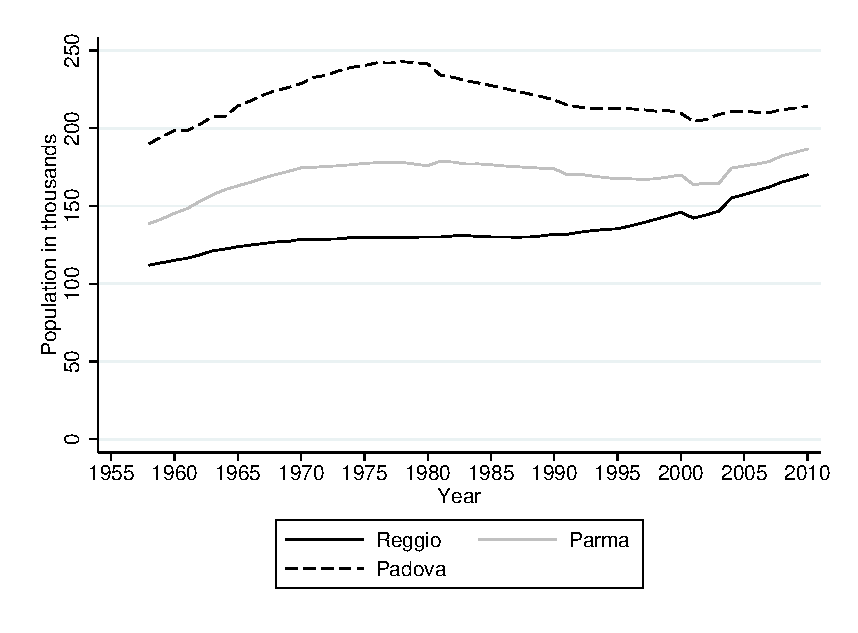
\includegraphics[width=\textwidth]{../../output/image/population.eps}
\caption{Population}
        \end{subfigure}
        \begin{subfigure}[t]{0.49\textwidth}
          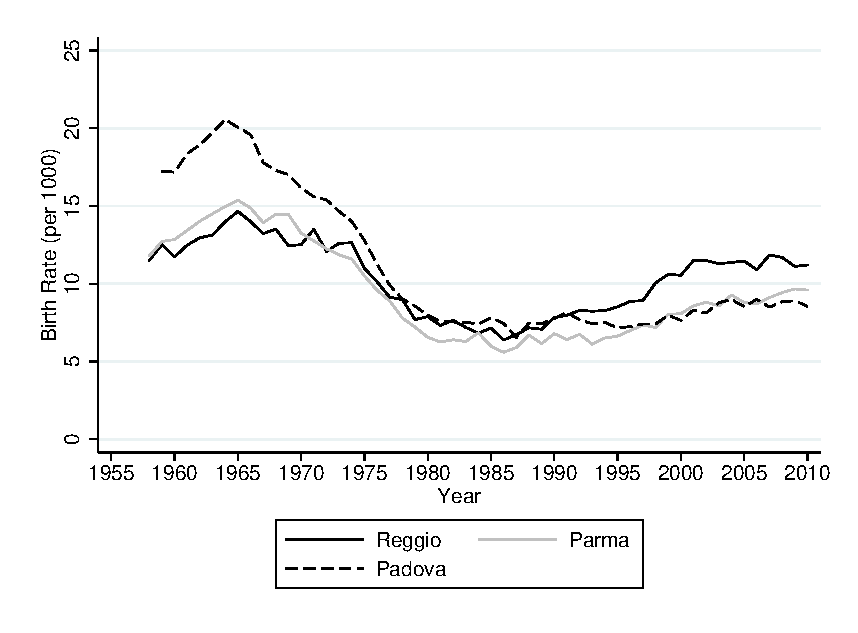
\includegraphics[width=\textwidth]{../../output/image/birth_rate.eps}
 \caption{Birth Rate}
        \end{subfigure}
        \begin{subfigure}[t]{0.49\textwidth}
          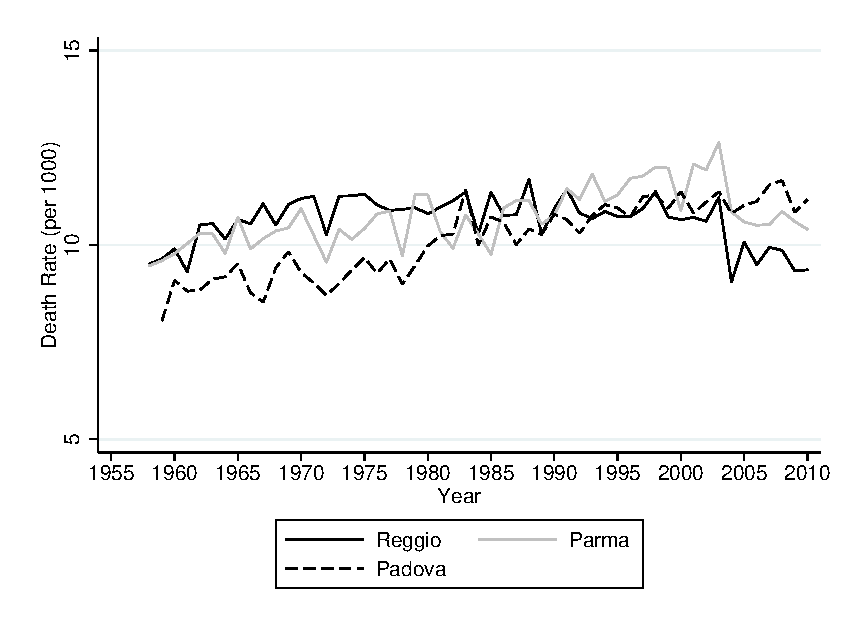
\includegraphics[width=\textwidth]{../../output/image/death_rate.eps}
        \caption{Death Rate}
        \end{subfigure}
        \begin{subfigure}[t]{0.49\textwidth}
          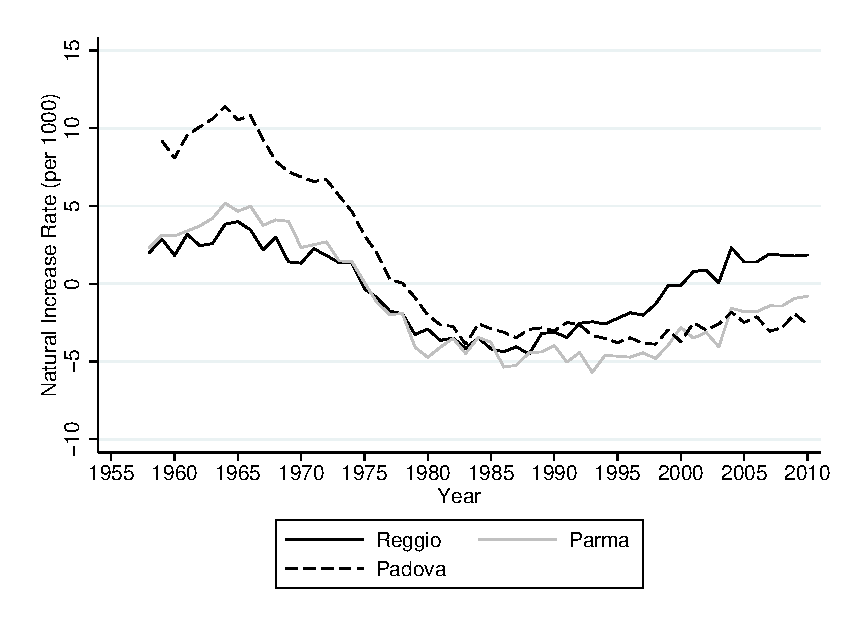
\includegraphics[width=\textwidth]{../../output/image/naturalinc_rate.eps}
            \caption{Natural Rate of Increase}
        \end{subfigure}
      \caption{Population Statistics}  \label{fig:population}
      \end{center}
      \raggedright Note: See Appendix~\ref{sec:data-app} for more information on these data and the sources.
    \end{figure}

\begin{figure}[H]
      \begin{center}
        \begin{subfigure}[t]{0.49\textwidth}
          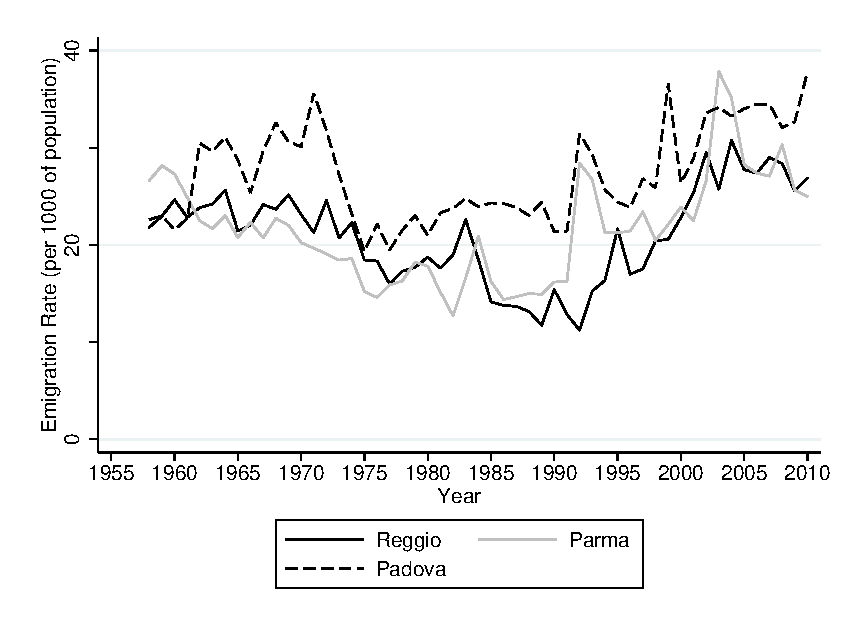
\includegraphics[width=\textwidth]{../../output/image/emigration.eps}
            \caption{Emigration}
        \end{subfigure}
      \begin{subfigure}[t]{0.49\textwidth}
        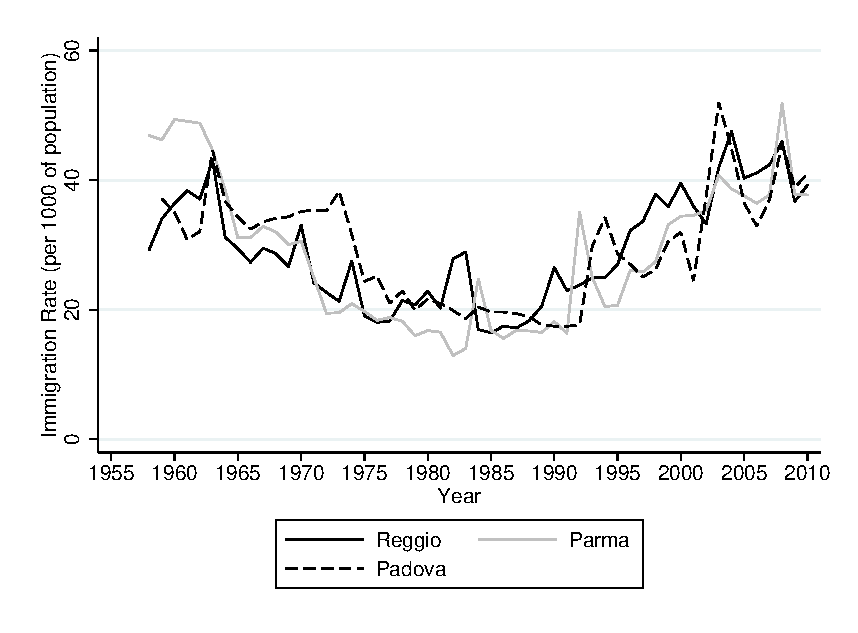
\includegraphics[width=\textwidth]{../../output/image/immigration.eps}
        \caption{Immigration}
      \end{subfigure}
	 \begin{subfigure}[t]{0.49\textwidth}
          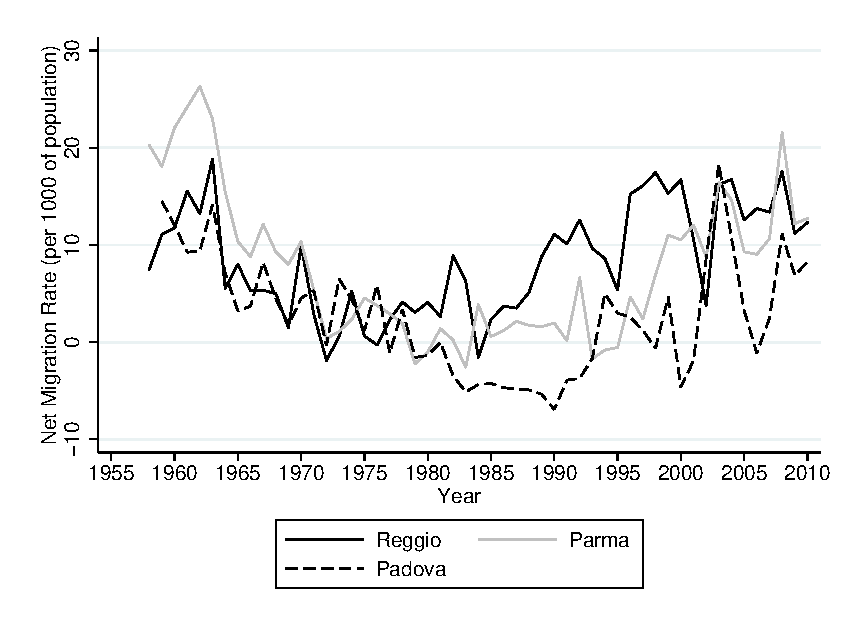
\includegraphics[width=\textwidth]{../../output/image/netmigration.eps}
\caption{Net Migration}
        \end{subfigure}
        \begin{subfigure}[t]{0.49\textwidth}
          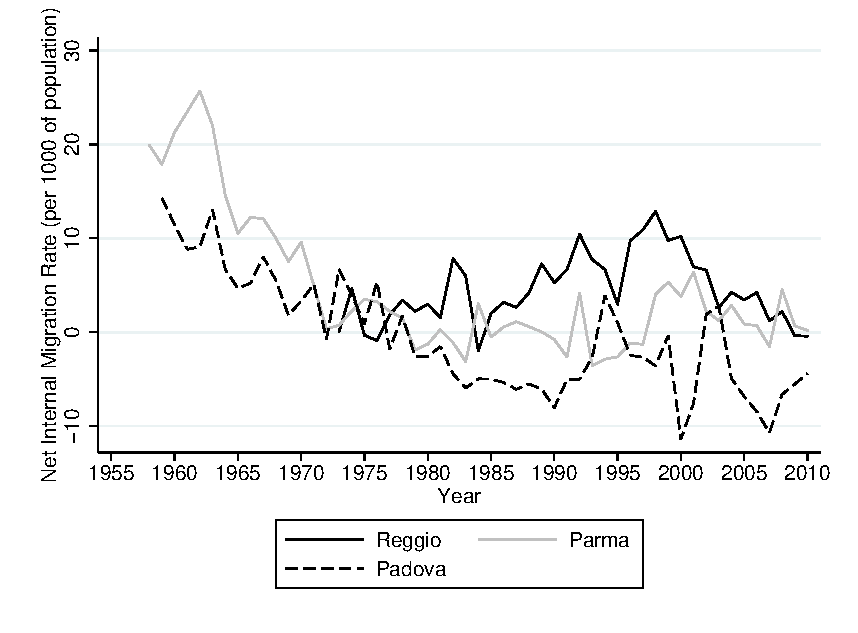
\includegraphics[width=\textwidth]{../../output/image/netinternalmig.eps}
 \caption{Net Internal Migration}
        \end{subfigure}
        \begin{subfigure}[ht]{0.48\textwidth}
          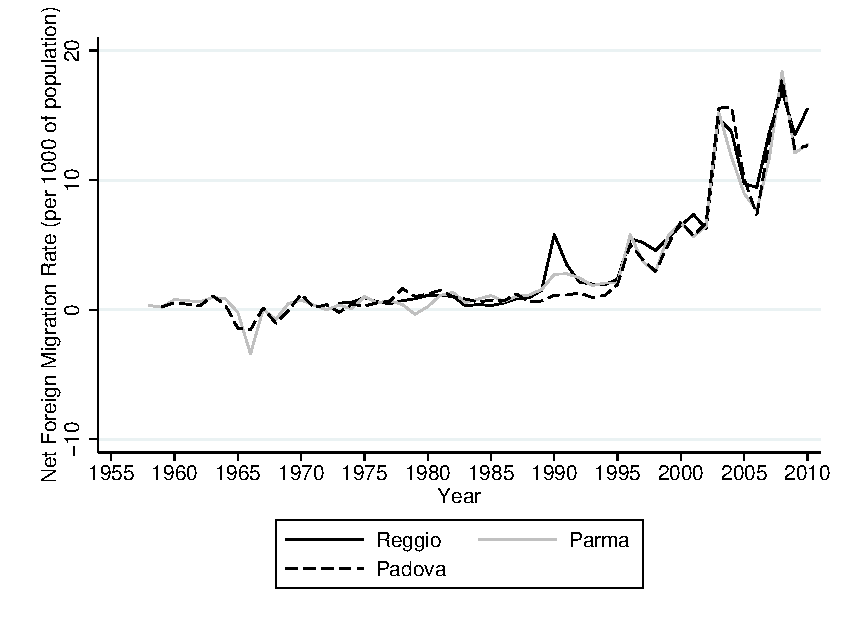
\includegraphics[width=\textwidth]{../../output/image/netforeignmig.eps}
        \caption{Net Foreign Migration}
        \end{subfigure}
      \caption{Migration Statistics}  \label{fig:emigr-immigr}
      \end{center}
         \raggedright  Note: See Appendix~\ref{sec:data-app} for more information on these data and the sources.
    \end{figure}

We summarize the main population statistics in Table~\ref{tab:pop-summary-stat} in which we present the mean and standard deviations of the population, birth rate, death rate, and net migration across years. We compare the means in Parma and Padova to those in Reggio Emilia. Parma and Padova have significantly larger populations.

    \begin{table}[H]
    \centering
    \caption{Summarizing Population Statistics Across Years} \label{tab:pop-summary-stat}
    \begin{threeparttable}
	
	\begin{tabular}{l c c c}
\toprule
&	Reggio Emilia & Parma & Padova \\
\midrule
Population	& 134,459.6 &   \textbf{170,335} &  \textbf{219,161.2}   \\
			& (13,413.67) & (10,104.85)& (13,474.66)   \\
Birth rate & 		10.38 &9.36  & 	11.08 \\
	(per 1,000)	&		(2.33) & (3.02) & (4.55) \\
Death rate &  10.62 &  10.74 & \textbf{10.13} \\
	(per 1,000)	& (0.63) & (0.74) & (095) \\
Net migration & 8.40 &  7.38 & \textbf{2.68} \\
	(per 1,000)		& (5.63) & (7.36) & (5.96) \\
\bottomrule
\end{tabular}


\begin{tablenotes}
\item \footnotesize Note: This table summarizes the average of population statistics across available years by city. A bolded mean indicates that it is significantly different from Reggio Emilia at least at the 0.05 level. Standard deviations are reported in parentheses. See Appendix~\ref{sec:data-app} for more information on these data and the sources.
\end{tablenotes}
\end{threeparttable}
\end{table}

Although the three cities are similar, Parma has more in common with Reggio Emilia than does Padova. This is the case for population indicators, such as those in Table~\ref{tab:pop-summary-stat}, but also for indicators of social setting. An example of this is seen in Appendix~\ref{sec:data-app} which has the proportion of votes for different parties between 1953 and 1993. In both Reggio Emilia and Parma, more votes went towards the Communist Party, whereas Padova had a higher proportion of votes going towards the Christian Democrats.

The proximity and comparability of the three cities are useful for standardizing on background variables. However, it may compromise sharp comparisons of the effectiveness of alternative school systems given the similarities in preschool features and commonality of cultural influences.
	
